\documentclass{utils/BachelorBUI}

\usepackage[utf8]{inputenc}
\RequirePackage[babel,austrian=quotes,english=american]{csquotes}

\raggedbottom

\lstset{
    language={Matlab},
}

\sisetup{output-decimal-marker = {,},
    range-phrase = --,
    group-separator = {~},
    per-mode = symbol,
    list-final-separator={ und }}

\graphicspath{{images/}}

\newcommand{\zB}{\mbox{z.\,B.}\xspace}
\newcommand{\Name}[1]{\textsc{#1}}

\newcommand{\vKTxv}{\mathbf{v}_1^T\tilde{\mathbf{K}}_{T},_{\xi}\mathbf{v}_1}
\newcommand{\vKTxxv}{\mathbf{v}_1^T\tilde{\mathbf{K}}_{T},_{\xi\xi}\mathbf{v}_1}

\usepackage[style=numeric-comp,backend=biber,maxcitenames=2]{biblatex}
\ExecuteBibliographyOptions{%
    giveninits=true,maxbibnames=99}%
\DefineBibliographyStrings{english}{%
    andothers={et\;al\adddot},
    urlseen={Accessed on\addcolon}
}
\DeclareFieldFormat{url}{%
    Available online\addcolon\space\url{#1}%
}
\addbibresource{utils/literature.bib}

\usepackage{acro}
\acsetup{list/display=used}

\usepackage{eurosym}

\DeclareAcronym{obv}{
short = {\"obv},
long  = {Österreichische Bautechnikvereinigung},
}

\DeclareAcronym{LZKB}{
short = {LZKB},
long  = {Lebenszykluskosten Brücken},
}

\DeclareAcronym{dt}{
short = {dt.},
long  = {deutsch},
}

\DeclareAcronym{abbv}{
short = {ABBV},
long  = {Ablösungsbeträge-Berechnungsverordnung},
short-plural = {s},
long-plural = {en},
}

\DeclareAcronym{lzk}{
short = {LZK},
long  = {Lebenszykluskosten},
extra = {[\officialeuro{}]},
}



\setcounter{biburllcpenalty}{9000}
\setcounter{biburlucpenalty}{9000}
\title{Schema-First Design of Forms in Web Apps: Integrating Angular, JsonForms and Spring Boot}
\authorname{Vlad-Ioan Dancea}
\email{danceavlad@icloud.com}
\MatrNr{12123455}
\thesislanguage{en-US}                        %% (de-AT, de-DE, en-GB, en-US)
\keywords{bachelor thesis\sep template\sep LaTeX}

\begin{document}

    \selectlanguage{english}

    \begin{filecontents}[overwrite]{\jobname.xmpdata}
        \makeatletter
        \Title{\@title}
        \Author{\@authorname}
        \Language{\@thesislanguage}
        \Keywords{\@keywords}
        \Publisher{TU Wien}
        \makeatother
    \end{filecontents}

    \maketitle

    %%%%%%%%%%%%%%%% Examples %%%%%%%%%%%%%%
    % Citation
    % \cite{Alberty:1999}

    % Footnote
    % \footnote{This is a footnote.}

    % Equation
    % \begin{equation}
    K_t
    =
    \left(
        1-
        \frac{R^2\cdot\tau}{c_a+\nu\cdot\tan\delta}
    \right)^4 \cdot k_1
    \label{Glg:Kt}
\end{equation}

    % Graphic
    % \usepackage{graphicx}
\begin{figure}[h]
    \centering{
        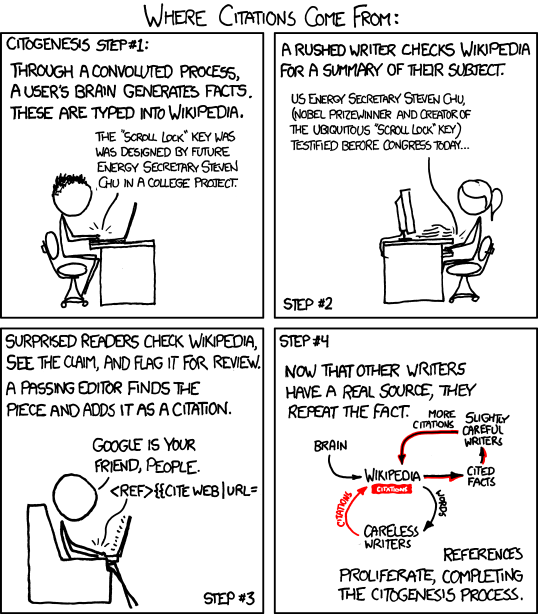
\includegraphics[width=9cm]{../images/citogenesis}
    }
    \caption{This is an example of a graphic}
    \label{fig:label:example-graphic}
\end{figure}

    % Table
    % \begin{table}[ht]
    \caption{The description comes above the table.
    Needs to be numbered.
    Last sentence without punctuation \label{tab:1}}
    \centering
    \begin{tabular}{lll}
        \toprule
        Column title 1 & Column title 2 & Column title 3 \\
        \midrule
        1  & 2  & 3  \\
        4  & 5  & 6  \\
        7  & 8  & 9  \\
        10 & 11 & 12 \\
        \bottomrule
    \end{tabular}
\end{table}

    % Code
    % \usepackage{listings}

\begin{lstlisting}[firstnumber=1,caption={Short caption},label={label}]
%FEM2D two-dimensional finite element method for Laplacian.
% Initialisation
load coordinates.dat; coordinates(:,1)=[];
eval('load elements3.dat; elements3(:,1)=[];','elements3=[];');
eval('load elements4.dat; elements4(:,1)=[];','elements4=[];');
eval('load neumann.dat; neumann(:,1) = [];','neumann=[];');
load dirichlet.dat; dirichlet(:,1) = [];
FreeNodes=@setdiff@(1:size(coordinates,1),unique(dirichlet));
A = sparse(size(coordinates,1),size(coordinates,1));
b = sparse(size(coordinates,1),1);

% Assembly
for j = 1:size(elements3,1)
  A(elements3(j,:),elements3(j,:)) = A(elements3(j,:),elements3(j,:)) ...
      + stima3(coordinates(elements3(j,:),:));
end
for j = 1:size(elements4,1)
  A(elements4(j,:),elements4(j,:)) = A(elements4(j,:),elements4(j,:)) ...
      + stima4(coordinates(elements4(j,:),:));
end
\end{lstlisting}
    %%%%%%%%%%%%%%%%%%%%%%%%%%%%%%%%%%%%%%%%

    \begin{abstract}
    Here comes the abstract of the thesis.
    It should be a short summary of the content of the thesis.
    It should contain at least 70 and at most 150 words.
    The font size should be 10pt.
    The left and right margins should be 1cm.
    The text in the abstract is written within the environment
    \texttt{\textbackslash{}begin\{abstract\}} and
    \texttt{\textbackslash{}end\{abstract\}}.
\end{abstract}

    \tableofcontents
    
    \section{Introduction}

The length of the Bachelor thesis is between 12 and 30 pages (excluding appendix).
After the title of the thesis, the author and a short abstract are given.
Then the main part of the thesis begins.
The Bachelor thesis has no title page and only an optional table of contents
(between abstract and chapter~1).

    \usepackage{listings}
\section{Background}

Before proposing and analyzing the new approach to form creation, it is important to understand the current state of
form development both in the context of the project and in general.

\subsection{Current Approach to Form Creation in Angular}

As highlighted in Angular's own documentation\cite{Angular:forms}, there are two main approaches to form creation, which
we will refer to as the \textit{template-driven} and \textit{reactive} approaches.
The consensus is that the template-driven approach is more suitable for simple forms, while the reactive approach is
better for complex forms.
We will focus on the reactive approach, as it is the one more suited for the project at hand, which requires complex
forms, but we will also briefly discuss the template-driven approach for completeness.

\subsubsection{Template-Driven Forms}

Template-driven forms are built largely in the component’s HTML template using the \texttt{FormsModule} directives such
as \texttt{ngModel}, \texttt{ngModelGroup,} and \texttt{ngForm}.
Every control in the template automatically creates an underlying \texttt{FormControl} instance, so there is minimal
TypeScript boilerplate.

A typical template-driven form might look like this:
\paragraph{HTML}
\begin{lstlisting}[language=HTML]
<form #form="ngForm" (ngSubmit)="onSubmit(form)">
  <div>
    <label for="name">Name</label>
    <input type="text" id="name" name="name" ngModel required>
  </div>
  <div>
    <label for="email">Email</label>
    <input type="email" id="email" name="email" ngModel email>
  </div>
  <button type="submit">Submit</button>
</form>
\end{lstlisting}

While quick to set up, this approach can become unwieldy as forms grow—implicit control creation hinders reuse, and
testing template logic is harder.

\subsubsection{Reactive Forms}

Reactive forms live in the component class as a defined data model (\texttt{FormGroup}, \texttt{FormControl}), offering
full control over validation, dynamic fields and testability.

\paragraph{HTML}
\begin{lstlisting}[language=HTML]
<form [formGroup]="contactForm" (ngSubmit)="onSubmit()">
  <div>
    <label for="name">Name</label>
    <input id="name" formControlName="name"/>
  </div>
  <div>
    <label for="email">Email</label>
    <input id="email" formControlName="email"/>
  </div>
  <button type="submit">Submit</button>
</form>
\end{lstlisting}

\paragraph{TypeScript}
\begin{lstlisting}[language=TypeScript]

  contactForm!: FormGroup;

  this.contactForm = new FormGroup({
    name: new FormControl('', [Validators.required]),
    email: new FormControl('', [Validators.required, Validators.email]),
    subscribe: new FormControl(false)
  });
\end{lstlisting}

Reactive forms provide:
\begin{itemize}
  \item \textbf{Dynamic fields:} ability to add or remove controls at runtime.
  \item \textbf{Explicit model:} full control over the form’s structure in TypeScript.
  \item \textbf{Testability:} ability to unit-test validation and control logic directly.
  \item \textbf{Type safety:} stronger guarantees with TypeScript typings.
\end{itemize}

In large‐scale applications like ours—with dynamic schemas, custom widgets and complex validation—reactive forms are
the recommended practice.

\subsection{Other Necessities}
In addition to the pure forms, the project requires many more features that heavily bloat the code, such as:

\begin{itemize}
  \item \textbf{Custom widgets:} Angular Material, PrimeNG, etc.
  \item \textbf{Validation:} both client-side and server-side.
  \item \textbf{State management:} for complex forms with multiple steps.
\end{itemize}

Before analyzing the new approach, these additional features must be considered, as they are essential for the
project and will influence the design of the new approach.

\subsubsection{Custom Widgets}

Angular provides a powerful suite of UI components through libraries like Angular Material and PrimeNG\@.
These components can be easily integrated into reactive forms, allowing for both prettier forms and a better user
experience.
Useful components include MatCard, MatInput, MatSelect, MatCheckbox and many more.
This, however, does not come without a cost, as it requires additional code to integrate these.
A standard approach using Angular Material might look like this:

\paragraph{HTML}
\begin{lstlisting}[language=HTML]
  <mat-card>
    <mat-card-content>
      <mat-form-field>
        <mat-label>Name</mat-label>
        <input matInput id="name" formControlName="name"/>
      </mat-form-field>
      <mat-form-field>
          <mat-label>Email</mat-label>
          <input matInput formControlName="email"/>
      </mat-form-field>
      <button mat-raised-button type="submit">Submit</button>
    </mat-card-content>
  </mat-card>
\end{lstlisting}

This extra wiring code adds to per-form boilerplate and motivates a schema-driven solution.

\subsubsection{Validation}

Validation is a crucial part of any form, and Angular provides a powerful validation framework that has two applications:
immediate client-side validation, which is shown to the user as they fill out the form, and the ability to also show
server-side validation errors, which are returned from the server after the form is submitted.
This is especially useful for complex forms where the server might have additional validation rules that cannot be easily
implemented on the client-side.
Thus using an error framework that supports both synchronous and asynchronous validation is essential.

Here is an example of how validation can be implemented in Angular with the MatError component:

\paragraph{HTML}
\begin{lstlisting}[language=HTML]
  <mat-form-field>
    <mat-label>Name</mat-label>
    <input matInput id="name" formControlName="name"/>
    @for (error of contactForm.controls['name'].errors; track error.message) {
      <mat-error>{{ error.message }}</mat-error>
    }
  </mat-form-field>
  <mat-form-field>
    <mat-label>Email</mat-label>
    <input matInput formControlName="email"/>
    @for (error of contactForm.controls['email'].errors; track error.message) {
      <mat-error>{{ error.message }}</mat-error>
    }
  </mat-form-field>
\end{lstlisting}

For each form control, we can define validation rules in the TypeScript code, which will be reflected in the HTML template.
But this leads to a lot of boilerplate and repetitive code, especially for large forms with many fields.

\subsubsection{State Management}

State management is another important aspect of complex forms, especially when dealing with multistep forms or forms
that require data to be shared between different components.
This can be achieved using popular libraries like NgRx or even with Angular's built-in signals.
Because the proposed approach also requires the developer to handmake components when NgRx or signals are used,
we will not go into detail about this, as it is not the focus of this thesis.
Suffice it to say that whatever state management is needed in the traditional approach, it will also be necessary in the
new approach.

Now that we have a good understanding of the current state of form creation in Angular, we can move on to analyzing the
problem with the current approach and the objectives of the new approach.

    \section{Problem Statement and Objectives}

\subsection{Problem Statement}
The current hands-on form development, while concrete and concise, is rigid and hard to adapt across projects.
Due to the requirement of the ability to change the appearance of the forms for each project user, the current approach
leads to many problems with the maintainability of the code.

Aside from the maintainability, the current approach also suffers from lots of redundancy in the code.
Forms share many common elements, such as labels, input fields, and buttons, yet the current approach duplicates code
rather than reusing components.

\subsection{Objectives}

With the problems clearly defined, the goal of this thesis is to analyze the feasibility of a new approach to form
creation, one that successfully addresses the problems of the current approach.
More specifically, the goals are:

\begin{itemize}
    \item To analyze how much boilerplate and duplication exist in the current form creation approach.
    \item To design a schema-driven approach that unifies the form creation logic and supports custom appearance for each
    project.
    \item To implement a prototype of the new approach and evaluate developer productivity and maintainability.
    \item To recommend whether the new approach is feasible for production use and the best approaches for going forward.
\end{itemize}

    \printbibliography

\end{document}